\documentclass{standalone}
\usepackage{pgfplots}
\pgfplotsset{compat=1.18}

\begin{document}
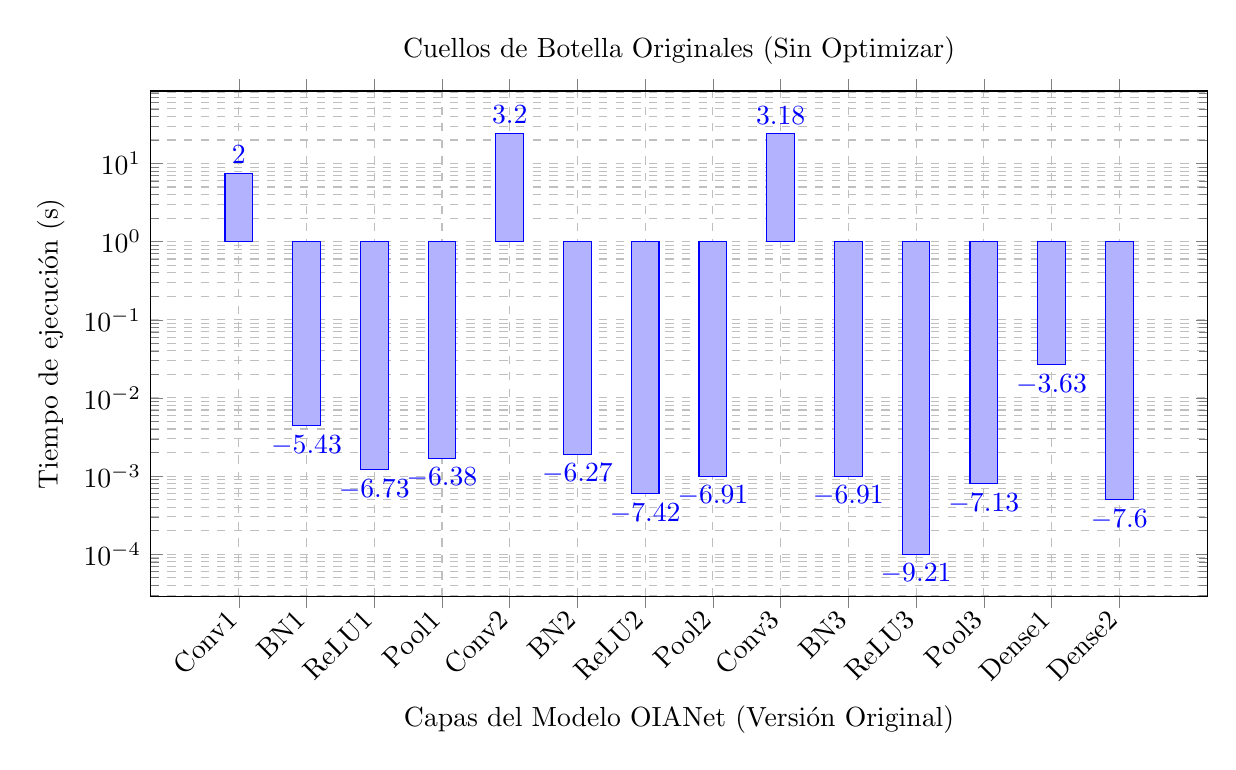
\begin{tikzpicture}
\begin{axis}[
    ybar,
    ymode=log,
    width=15cm,
    height=8cm,
    ylabel={Tiempo de ejecución (s)},
    xlabel={Capas del Modelo OIANet (Versión Original)},
    xtick=data,
    xticklabels={Conv1, BN1, ReLU1, Pool1, Conv2, BN2, ReLU2, Pool2, Conv3, BN3, ReLU3, Pool3, Dense1, Dense2},
    x tick label style={rotate=45, anchor=east},
    nodes near coords,
    nodes near coords align={vertical},
    title={Cuellos de Botella Originales (Sin Optimizar)},
    grid=both,
    grid style={dashed}
]
\addplot coordinates {
    (1, 7.4059)
    (2, 0.0044)
    (3, 0.0012)
    (4, 0.0017)
    (5, 24.5160)
    (6, 0.0019)
    (7, 0.0006)
    (8, 0.0010)
    (9, 23.9566)
    (10, 0.0010)
    (11, 0.0001)
    (12, 0.0008)
    (13, 0.0265)
    (14, 0.0005)
};
\end{axis}
\end{tikzpicture}
\end{document}
